%\documentclass[10pt, a4paper]{report}
%\begin{document}
%This is an % stupid
%% Better: instructive <----
%example: Supercal%
%ifragilist%
%icexpialidocious
%\end{document}

%% our first LaTex Example!
%\documentclass{article}
%\begin{document}
%Hello World!
%\end{document}

%\documentclass[11pt, a4paper]{report}
%\begin{document}{doublespace}{1.6}
%\title{How to structure a LaTex Document}
%\author{AVIRAL Anand}
%\date{\today}
%\maketitle
%\begin{abstract}
%Wombat\textsubscript{walzing}
%This is a paragraph with a very long word ABCDEFGHJ framed on March 10\textsuperscript{th}, 1999;then we have an another bad thing, a long number 1234567890123456789
%\end{abstract}
%\end{document}{doublespace}{1.6}

%\documentclass[12pt, a4paper]{report}
%\begin{document}
%My name is \ldots Aviral Mangal.\\
%Hyphen: daughter-in-law, X-rated\\
%En dash: pages 13--67\\
%Em dash: yes---or no? \\
%Minus sign: $0$, $1$ and $-1$
%\end{document}

%\documentclass[12pt, a4paper]{report}
%\begin{document}
%\begin{verbatim}
%My name is \ldots Aviral Mangal.\\
%     Hyphen: daughter-in-law, X-rated\\
%En dash:        pages 13--67\\
%     Em dash: yes---or no? \\
%Minus sign: $0$, $1$ and $-1$
%The verbatim environment
%simply reproduces every
%character you input,
%including all s p a c e s!
%\end{verbatim}
%\end{document}

%error in using the below code
%\usepackage{alltt}
%\documentclass[12pt, a4paper]{report}
%\begin{document}
%\begin{alltt}
%Verbatim extended with the ability
%to use normal commands. Therefore, it
%is possible to \emph{emphasize} words in
%this environment, for example.
%\end{alltt}
%\end{document}

%\documentclass[12pt, a4paper]{report}
%\begin{document}
%\textbf
%{This is another
%\begin{LARGE}
%\textit{rather stupid,
%but helpful}
%\end{LARGE}
%example for embedding
%comments in your document.}
%\end{document}

%\documentclass{article}
%\usepackage{blindtext}
%\begin{document}
%\begin{itemize}
%\item \blindtext
%\item \blindtext
%\end{itemize}
%\begin{enumerate}
%\item \blindtext
%\item \blindtext
%\end{enumerate}
%\begin{description}
%\item [Ant] \blindtext
%\item [Elephant] \blindtext
%\end{description}
%\end{document}

%\documentclass{article}
%\usepackage{blindtext}
%\begin{document}
%\begin{itemize}
%\item \blindtext
%\item \blindtext
%\end{itemize}
%\begin{enumerate}
%\item \blindtext
%\item \blindtext
%\end{enumerate}
%\begin{description}
%\item [Ant] \blindtext
%\item [Elephant] \blindtext
%\end{description}
%\end{document}

%\documentclass[12pt, a4paper]{article}
%\begin{document}
%\begin{enumerate}
%\item The first item
%\begin{enumerate}
%\item Nested item 1
%\item Nested item 2
%\end{enumerate}
%\item{ The second item}
%\item The third etc \ldots
%\end{enumerate}
%\end{document}

%\documentclass[twocolumn]{article}
%\usepackage{blindtext}
%\usepackage{scrextend}
%\addtokomafont{labelinglabel}{\sffamily}
%\begin{document}
%\blindtext
%\begin{labeling}{alligator}
%\item [ant] really busy all the time
%\item [chimp] likes bananas
%\item [alligator] very dangerous animal, sharp teeth, long
%muscular tail and a bit of text that is longer than one
%line and shows the alignment of text quite nicely
%\end{labeling}
%\end{document}

%\documentclass[twocolumn]{article}
%\usepackage{blindtext}
%\usepackage[inline]{enumitem}
%\usepackage{xcolor}
%\begin{document}
%\blindtext Coco likes fruit. Her favorites are : 
%\begin{enumerate*}[label = {\alph*)}, font = {\color{red!50!black}\bfseries}]
%\item bananas
%\item apples
%\item oranges and
%\item lemons.
%\end{enumerate*}
%\blindtext
%\end{document}

%\documentclass{article}
%\usepackage{blindtext}
%\usepackage{tasks}
%\begin{document}
%Which one of the entries does not fit with the others?
%\begin{tasks}(4)
%\task mercury
%\task iron
%\task lead
%\task zinc
%\end{tasks}
%\end{document}

%\documentclass[twocolumn]{article}
%\usepackage{blindtext}
%\usepackage{enumitem}
%\begin{document}
%\blindtext
%\begin{itemize}
%\item more work
%\item more responsibility
%\item more satisfaction
%\end{itemize}
%\blindtext
%\newpage
%\blindtext
%\begin{itemize}[noitemsep]
%\item more work
%\item more responsibility
%\item more satisfaction
%\end{itemize}
%\blindtext
%\end{document}


% An example for alignment and width of the label
%\documentclass[twocolumn]{article}
%\usepackage{blindtext}
%\usepackage{enumitem}
%\begin{document}
%\blindtext Coco likes fruit. Her favourites are:
%\begin{description}[align=left]
%\item [Kate] some detail
%\item [Chris]some detail
%\item [Laura]some detail
%\end{description}
%\begin{description}[align=right]
%\item [Kate] some detail
%\item [Christina]some detail
%\item [Laura]some detail
%\end{description}
%\begin{description}[align=right,labelwidth=3cm]
%\item [Kate] some detail
%\item [Christina]some detail
%\item [Laura]some detail
%\end{description}
%\blindtext
%\end{document}

%\documentclass[12pt, a4paper]{article}
%\usepackage{amsmath}
%\usepackage{siunitx}
%\begin{document}
%It is $\SI{17}{\degreeCelsius}$ outside.
%\end{document}


%\documentclass[12pt, a4paper]{article}
%\usepackage{rotating}

%\documentclass[12pt, a4paper]{article}
%\begin{document}
%\begin{tabular}{l c r}
%1 & 2 & 3 \\
%4 & 5 & 6 \\
%7 & 8 & 9 \\
%\end{tabular}
%\end{document}

%% including some vertical lines
%\documentclass[12pt, a4paper]{article}
%\begin{document}
%\begin{tabular}{ l | c || r }
%1 & 2 & 3 \\
%4 & 5 & 6 \\
%7 & 8 & 9 \\
%\end{tabular}
%\end{document}


%% to add horizontal lines to the very top and bottom of the table
%\documentclass[12pt, a4paper]{article}
%\begin{document}
%\begin{tabular}{l | c || r}
%\hline
%1 & 2 & 3 \\
%4 & 5 & 6 \\
%7 & 8 & 9 \\
%\hline
%\end{tabular}
%\end{document}


%\documentclass[12pt, a4paper]{article}
%\begin{document}
%\begin{tabular}{l | c || r}
%\hline
%1 & 2 & 3 \\
%\hline
%4 & 5 & 6 \\
%\hline
%7 & 8 & 9  \\
%\hline
%\end{tabular}
%\end{document}


%\documentclass[12pt, a4paper]{article}
%\begin{document}
%\begin{tabular}{l | c ||| r}
%\hline
%1 & 2 & 3 \\
%\hline
%4 & 5 & 6 \\
%\hline \hline
%7 & 8 & 9  \\
%\hline
%\end{tabular}
%\end{document}


%\documentclass[12pt, a4paper]{article}
%\begin{document}
%\begin{tabular}{l | c | r}
%\hline
%7C0 & hexadecimal \\
%3700 & octal \\ \cline{2-2}
%11111000000 & binary \\
%\hline \hline
%1984 & decimal \\
%\hline
%\end{tabular}
%\end{document}




%\documentclass{article}
%\usepackage[english]{babel}
%\begin{document}
%Without specifying width for last column:
%\begin{center}
%\begin{tabular}{l l l l } 
%\hline
%Day & Min Temp & Max Temp & Summary \\ \hline
%Monday & 11C & 22C & A clear day with lots of sunshine.
%However, the strong breeze will bring down the temperatures. \\ \hline
%Tuesday & 9C & 19C & Cloudy with rain, across many northern regions. Clear
%spells
%across most of Scotland and Northern Ireland,
%but rain reaching the far northwest. \\ \hline
%Wednesday & 10C & 21C & Rain will still linger for the morning.
%Conditions will improve by early afternoon and continue
%throughout the evening. \\
%\hline
%\end{tabular}
%\end{center}
%With width specified:
%\begin{center}
%\begin{tabular}{ l l l p{5cm} }
%\hline
%Day & Min Temp & Max Temp & Summary \\ \hline
%Monday & 11C & 22C & A clear day with lots of sunshine.
%However, the strong breeze will bring down the temperatures. \\ \hline
%Tuesday & 9C & 19C & Cloudy with rain, across many northern regions. Clear spells across most of Scotland and Northern Ireland, but rain reaching the far northwest. \\ \hline
%Wednesday & 10C & 21C & Rain will still linger for the morning.
%Conditions will improve by early afternoon and continue
%throughout the evening. \\
%\hline
%\end{tabular}
%\end{center}
%\end{document}



%\documentclass{article}
%\usepackage[english]{babel}
%\begin{document}
%\begin{tabular}{cc}
%boring cell content & \parbox[t]{5cm}{rather long par\\new par}
%\end{tabular}
%\end{document}



%%Spacing between rows
%\documentclass{article}
%\begin{document}
%\begin{tabular}{ l l r }
%\hline \noalign{\smallskip}
%\multicolumn{2}{c}{Item} \\
%\cline{1-2}\noalign{\smallskip}
%Animal & Description & Price(\$) \\
%\noalign{\smallskip}\hline\noalign{\smallskip}
%Gnat & per gram & 13.65 \\
%     & each     & 0.01 \\
%Gnu  & stuffed  & 92.50 \\
%Emu  & stuffed  & 33.33 \\
%Armadillo & frozen & 8.99 \\
%\noalign{\smallskip}\hline
%\end{tabular}
%\end{document}
       

%% Defining multiple columns in a table       
%\documentclass{article}
%\begin{document}
%\begin{tabular}{l*{6}{c}r}
%Team                 & P & W & D & L & F & A & Pts \\
%\hline
%Manchester United    & 6 & 4 & 0 & 2 & 10 & 5 & 12 \\
%Celtic               & 6 & 3 & 0 & 3 & 8 & 9 & 9 \\
%Benfica              & 6 & 2 & 1 & 3 & 7 & 8 & 7 \\
%FC Copenhagen        & 6 & 2 & 1 & 3 & 5 & 8 & 7 \\
%\end{tabular}
%\end{document}       



%\documentclass{article}
%\begin{document}
%\begin{tabular}{l*{6}{c}r}
%Team & P & W & D & L & F & A & Pts \\
%\hline
%Manchester United & 6 & 4 & 0 & 2 & 10 & 5 & 12 \\
%Celtic & 6 & 3 & 0 & 3 & 8 & 9 & 9 \\
%Benfica & 6 & 2 & 1 & 3 & 7 & 8 & 7 \\
%%FC Copenhagen & 6 & 2 & 1 & 3 & 5 & 8 & 7 \\
%\end{tabular}
%\end{document}


%% Aligning columns at decimal points using dcolumn
%\documentclass{article}
%\usepackage{dcolumn}
%\begin{document}
%%\ldots
%\newcolumntype{d}[1]{D{.}{\cdot}{#1} }
%%the argument for d specifies the maximum number of decimal places
%\begin{tabular}{l r c d{1} }
%Left&Right&Center&\mathrm{Decimal}\\
%1&2&3&4\\
%11&22&33&44\\
%1.1&2.2&3.3&4.4\\
%\end{tabular}
%\end{document}


%% Bold text and dcolumn
%\documentclass{article}
%\usepackage{dcolumn}
%%here we're setting up a version of the math fonts with normal x-width
%\DeclareMathVersion{nxbold}
%\SetSymbolFont{operators}{nxbold}{OT1}{cmr} {b}{n}
%\SetSymbolFont{letters} {nxbold}{OML}{cmm} {b}{it}
%\SetSymbolFont{symbols} {nxbold}{OMS}{cmsy}{b}{n}
%\begin{document}
%\makeatletter
%\newcolumntype{d}{D{.}{.}{-1}}   %decimal columns as before
%%wide bold decimal column
%\newcolumntype{B}[3]{>{\boldmath\DC@{#1}{#1}{#3}}c<{\DC@end}}
%\makeatother
%\begin{tabular}{l l d}
%Type &M & \multicolumn{1}{c}{N} \\
%Normal & 1 & 2222.222 \\
%Bold(standard) &10 & \multicolumn{1}{B{.}{.}{-1} }{2222.222} \\
%Bold (nxbold) &100 & \multicolumn{1}{B{.}{.}{-1} }{2222.222} \\
%\end{tabular}
%\end{document}


%% Row spanning multiple columns
%\documentclass{article}
%\begin{document}
%\begin{tabular}{ ll }
%\hline
%\multicolumn{2}{Team sheet} 
%{
%\\
%GK & Paul Robinson \\
%LB & Lucas Radebe \\
%DC & Michael Duberry \\
%DC & Dominic Matteo \\
%RB & Dider Domi \\
%MC & David Batty \\
%MC & Eirik Bakke \\
%MC & Jody Morris \\
%FW & Jamie McMaster \\
%ST & Alan Smith \\
%ST & Mark Viduka \\
%\hline
%\end{tabular}
%\end{document}


%% Rows spanning multiple columns
%\documentclass{article}
%\begin{document}
%\begin{tabular}{ l l}
% \hline
% \multicolumn{2}{c}{Team Sheet} \\
% \hline 
%GK & Paul Robinson \\
%LB & Lucas Radebe \\
%DC & Michael Duberry \\
%DC & Dominic Matteo \\
%RB & Dider Domi \\
%MC & David Batty \\
%MC & Eirik Bakke \\
%MC & Jody Morris \\
%FW & Jamie McMaster \\
%ST & Alan Smith \\
%ST |& Mark Viduka \\
%\hline
%\end{tabular}
%\end{document}


%%Columns spanning multiple rows\
%\documentclass{article}
%\usepackage{multirow}
%\begin{document}
%\begin{tabular}{l l l}
%\hline
%\multicolumn{3}{c}{Team sheet} \\
%\hline
%Goalkeeper & GK & Paul Robinson \\ \hline
%\multirow{4}{*}{Defenders} & LB & Lucas Redebe \\
%& DC & Michael Duburry \\
%& DC & Dominic Matteo\\
%& RB & Didier Domi \\ \hline
%\multirow{3}{*}{Midfielders} & MC & David Batty \\
%& MC & Eirik Bakke \\
%& MC & Jody Morris \\ \hline
%Forward & FW & Jamie McMaster \\ \hline
%\multirow{2}{*}{Strikers} & ST & Alan Smith \\
%& ST & Mark Viduka \\
%\hline
%\end{tabular}
%\end{document}
%
%\end{tabular}


%% Spanning in both directions simultaneously
%\documentclass{article}
%\usepackage{multirow}
%\begin{document}
%\begin{tabular}{ccccccl}
%& & \multicolumn{4}{c}{Primes} \\ \cline{3-6}
%& & 2 & 3 & 5  & 7 \\ \cline{1-6}
%\multicolumn{1}{c}{\multirow{2}{*}{Powers}} &
%\multicolumn{1}{c}{504} & 3 & 2 & 0 & 1 & \\ \cline{2-6}
%\multicolumn{1}{c}{}                      &
%\multicolumn{1}{c}{540} & 2 & 3 & 1 & 0 & \\ \cline{1-6}
%\multicolumn{1}{c}{\multirow{2}{*}{Powers}} &
%\multicolumn{1}{c}{gcd} & 2 & 2 & 0 & min \\ \cline{2-6}
%\multicolumn{1}{c}{}                       &
%\multicolumn{1}{c}{lcm} & 3 & 3 & 1 & 1 & max \\ \cline{1-6}
%\end{tabular}
%\end{document}   
%\end{tabular}


%\documentclass{article}
%\begin{document}
%\begin{tabular}{ r c c}
%\multicolumn{1}{r}{}
%& \multicolumn{1}{c}{noninteractive}
%& \multicolumn{1}{c}{interactive} \\
%\cline{2-3}
%massively multiple & Library & University \\
%\cline{2-3}
%one-to-one & Book & Tutor \\
%\cline{2-3}
%\end{tabular}
%\end{document}

%
%% Resizing table including the caption
%
%\documentclass{article}
%\usepackage{graphicx}
%\begin{document}
%\begin{table}[h]
%\resizebox{1.4\textwidth}{!}{\begin{minipage}{\textwidth}
%\begin{tabular}{r c c}
%& \multicolumn{1}{c}{noninteractive}
%& \multicolumn{1}{c}{interactive} \\
%\cline{2-3}
%massively multiply & Library & University \\
%\cline{2-3}
%one-to-one & Book & Tutor \\
%\cline{2-3}
%\end{tabular}
%\caption[Table caption text]{Table taken from \cite[p.10]}
%\label{table:name}
%\end{minipage}
%\end{table}
%\end{document}



%% Normal LaTeX table
%\documentclass{article}
%\begin{document}
%\begin{tabular}{l l r}
%\hline
%\multicolumn{2}{c}{Item} \\
%\cline{1-2}
%Animal & Description & Price (\$) \\
%\hline
%Gnat   & per gram    & 13.65       \\
%       & each        & 0.01        \\
%Gnu    & stuffed     & 92.50       \\
%Emu    & stuffed     & 33.33       \\
%Armadillo & frozen   & 8.99      \\
%\hline
%\end{tabular}
%\end{document}


%% Using array package for table creation
%\documentclass{article}
%\usepackage{array}
%\begin{document}
%\begin{tabular}{l l r}
%\firsthline
%\multicolumn{2}{c}{Item}  \\
%\cline{1-2}
%Animal  & Description & Price (\$) \\
%\hline
%Gnat    & per gram    & 13.65     \\
%        & each        & 0.01     \\
%Gnu     & stuffed     & 92.50    \\
%Emu     & stuffed     & 33.33    \\
%Armadillo & frozen    & 8.99      \\
%\lasthline      
%\end{tabular}
%\end{document}



%% Title creation
%\documentclass[12pt, a4paper]{report}
%\usepackage{graphicx}
%\graphicspath{{C:/Users/PC/Desktop/}}
%\begin{document}
%\begin{titlepage}
%     \centering 
%   %  \includegraphics[width = 0.15\textwidth]{example-image-1x1}\par
%   
\includegraphics[scale = 0.75, width = 70pt, keepaspectratio = true]{DEI0logo.jpg} \par
%   \vspace{1cm}
%     {\scshape\LARGE Columbidae University \par}
%     \vspace{1cm}
%     {\scshape\Large Final year project\par}
%     \vspace{1.5cm}
%     {\huge\bfseries Pigeons love doves \par}
%     \vspace{2cm}
%     {\Large\itshape John Birdwatch \par}
%     \vfill
%     supervised by\par
%     Dr. ~Mark \textsc{Brown}
%     \vfill
%% Bootom of the page     
%     {\large \today\par}    
%\end{titlepage}
%\end{document}


%\documentclass[12pt, a4paper]{report}
%\usepackage{graphicx}
%\graphicspath{{C:/Users/PC/Desktop/}}
%\begin{document}
%\begin{titlepage}
%     \centering
%      
\includegraphics{DEI0logo.jpg}
%\vspace{1cm}
%\end{titlepage}     
%\end{document}


%% Images as figures
%\documentclass[12pt, a4paper]{article}
%\usepackage{graphicx}
%\begin{document}
%\begin{figure}[p]
% \centering
% 
\includegraphics{DEI0logo.jpg}
% \caption{Awesome Image}
% \label{fig:awesome_image}
%\end{figure}
%\end{document}



%% Seamless text integration
%\documentclass[12pt, a4paper]{article}
%\usepackage{graphicx}
%\begin{document}
%\fbox{\setlength{\unitlength}{0.8cm}
%\begin{picture}(6,5)
%\put(3.5, 0.4){$\displaystyle
%s: = \frac{a + b + c}{2}$}
%\put(1,1){
\includegraphics[width = 2cm, height = 2cm]{DEI0logo.jpg}}    
%\end{picture}  }
%\end{document}



%\documentclass[a4paper, 12pt]{report}
%\usepackage[english]{babel}
%\usepackage{graphicx}
%\begin{document}
%\begin{figure}[!ht]
%   \caption{A picture of a gull.} 
%   \vspace{1cm}
%   \centering
%     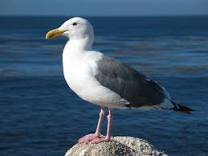
\includegraphics[width = 0.10\textwidth]{gull.jpg} 
%     \vspace{1cm}
%\end{figure}
%
%\begin{figure}[!ht]
%  \centering
%    \reflectbox{%
%      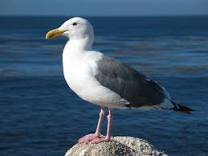
\includegraphics[width = 0.10\textwidth]{gull.jpg} < !---->}
%  \caption{A picture of the same gull looking the other way!}
%\end{figure}
%      
%\begin{table}[!ht]
%  \begin{center}
%    \begin{tabular}{l c r}
%    \hline
%    1 & 2 & 3 \\
%    4 & 5 & 6 \\
%    7 & 8 & 9 \\
%    \hline
%    \end{tabular}
%  \end{center}
%  \caption{A simple table}
%\end{table}     
%    
%Notice how the tables and figures have independent counters.
%\end{document}



% Side caption

%\documentclass{article}
%\usepackage{graphicx}
%\usepackage{sidecap}
%\begin{document}
%\begin{SCfigure}
% \centering
% \caption{..... caption text ....}
% \vspace{1cm}
% 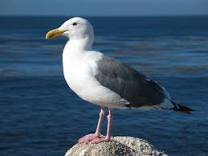
\includegraphics[width = 0.3\textwidth]{gull.jpg}
%\end{SCfigure}
%\end{document}
%  



%%wrapping text
%\documentclass[12pt, a4paper]{article}
%\usepackage{graphicx}
%\usepackage{wrapfig}
%\begin{document}
%\begin{wrapfigure}{r}{0.5\textwidth}
%  \begin{center}
%   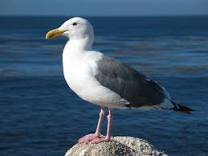
\includegraphics[width = 0.48\textwidth]{gull.jpg}
%  \end{center}
%  \caption{A gull}
%\end{wrapfigure}  
%\end{document}



%\documentclass[12pt, a4paper]{article}
%\usepackage{graphicx}
%\usepackage[english]{babel}
%\usepackage{caption}
%\usepackage{subcaption}
%\begin{document}
%\begin{figure}[!ht]
%  \begin{minipage}{\textwidth}
%  \centering
%  \begin{subfigure}[b]{0.3\textwidth]
%    
\includegraphics[width = \textwidth]{DEI0logo.jpg}
%    \caption{Dayalbagh Educational Institute}
%    \label{fig: DEI0logo.jpg}  
%  \end{subfigure}  
%  \begin{subfigure}[b]{0.3\textwidth}
%    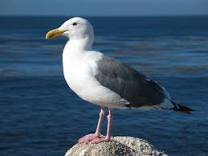
\includegraphics[]{gull.jpg}
%    \caption{A gull}
%    \label{fig: gull.jpg}
%  \end{subfigure}
%  \begin{subfigure}[b]{0.3\textwidth]
%    
\includegraphics[width = \textwidth]{DEI0logo.jpg}
%    \caption{Dayalbagh Educational Institute}
%    \label{fig: DEI0logo.jpg}  
%  \end{subfigure}  
%  \caprion{Something mad done by Aviral}\label{fig:just like that}
%  \end{minipage}   
%\end{figure}
%\end{document}


%\documentclass[12pt, a4paper]{article}
%\usepackage{mathtools}
%\usepackage{amsmath}
%\usepackage{xfrac}
%
%\begin{document}
%\begin{align*}
%\forall x \in X, \quad \exists y \leq \epsilon \\
%
%\cos (2\theta) = \cos^2 \theta - \sin^2 \theta \\
%
%\lim_{x \to \infty} \exp(-x) = 0 \\
%
%% a mod b
%a \bmod b
%
%x \equiv a \pmod b
%
%k_{n+1} = n^2 + k_n^2 - k_{n-1}
%
%%For powers with more than one digit, surround the power with {}.
%n^{22}
%
%%An underscore (_) can be used with a vertical bar (|) to denote evaluation using subscript notation in mathematics
%f(n) = n^5 + 4n^2 + 2_{n=17}
%
%\begin{equation}
%\frac{n!}{k!(n-k)!} = \binom{n}{k}
%\end{equation}
%
%\begin{equation}
%\frac{n!}{k!(n-k)!} = {n \choose k}
%\end{equation}
%
%%You can embed fractions within fractions:
%\begin{equation}
%\frac{\frac{1}{x} + \frac{1}{y}}{y-z}
%\end{equation}
%
%Take $\sfrac{1}{2}$ cup of sugar, \dots
%3\times\sfrac{1}{2}=1\sfrac{1}{2}
%
%\begin{equation}
%x = a_0 + \cfrac{1}{a_1
%+ \cfrac{1}{a_2
%+ \cfrac{1}{a_3 + \cfrac{1}{a_4} } } }
%\end{equation}
%
%\sqrt{\frac{a}{b}}
%
%\sqrt[n]{1+x+x^2+x^3+\ldots}
%
%\sum_{i=1}^{10} t_i
%
%\displaystyle\sum_{i=1}^{10} t_i
%\end{align*}
%\end{document}




\documentclass[12pt]{report}
\usepackage{amsmath}
\begin{document}
\begin{align*}
  f(x) &= x^4 + 7x^3 + 2x^2 \\
  &\qquad {} + 10x + 12
\end{align*}  
\begin{align}
  f(x) &= x^4 + 7x^3 + 2x^2 \nonumber \\
  &\qquad {} + 10x + 12
\end{align}
\begin{align*}
 f(x)  &= ax^2 + bx + c    &  g(x) &= dx^3 \\
 f'(x) &= 2ax + b          &  g'(x) &= 3dx^2  
\end{align*}
%Braces spanning multiple lines
\begin{align}
 f(x) &= \pi \left\{x^4 + 7x^3 + 2x^2 \right.\nonumber \\
 &\qquad \left. {} + 10x + 12 \right\}
\end{align}
\[
u(x) =
\begin{cases}
\exp{x} & \text{if } x \geq 0 \\
1 & \text{if } x < 0
\end{cases}
\]
\[
f(x) =
\begin{cases}
x & \text{when} x \text{is even} \\
-x & \text{when} x \text{is odd}
\end{cases}
\]
\begin{equation}
\lim_{a\to \infty} \frac{1}{a}
\end{equation}
\begin{equation}
\frac{n!}{k!(n-k)!} = {n \choose k}
\end{equation}
\begin{equation}
\frac{n!}{k!(n-k)!} = \binom{n}{k}
\end{equation}
\begin{equation}
x = a_0 + \frac{1}{\displaystyle a_1
+ \frac{1}{\displaystyle a_2
+ \frac{1}{\displaystyle a_3 + a_4}<!-- -->}<!-- -->}
\end{equation}
\end{document}